\chapter{Variationsprinzip}
Es gibt viele Ansätze den Hamiltonian des Zentralspinmodells zu lösen, die von der exakten Lösung über 
semiklassischen Ansätzen\cite{PhysRevB.65.205309,PhysRevB.94.094308,PhysRevB.70.205327,NatalieJaeschke} bishin zum
Chebychev Expansionstheorem reichen\cite{PhysRevB.89.045317}, welche ihre eigenen Vor- und Nachteile beherbergen. 
Gerade bei einer großen Anzahl von Kernspins ist eine exakte quantenmechanische Lösung nicht anwendbar. Deshalb finden semiklassische Ansätze Verwendung, 
die eine Abweichung zur exakten Lösung in Kauf nehmen, um dafür mehr Spins behandeln zu können. In dieser Arbeit wird das Time-Dependent Variatonal 
Principle, kurz TDVP, zur Lösung verwendet. Im folgenden werden komplex konjugierte Variablen $\muk$ mit einem Oberbalken notiert.

\textbf{Historische Randnotiz}\\
Dirac (1930) hat als Erster das Variationsprinzip zur Lösung der zeitabhängigen Schrödingergleichung unter unkommentierten Annahmen vorgestellt; 
diese Annahmen sind in P. A. M. Dirac "Mathematical Proceedings of the Cambridge Philosophical Society 26, 376 (1930)"\cite{Dirac1930-fc} 
zu finden und werden im Rahmen dieser Bachelorarbeit nicht explizit erläutert. \\
Viele Physiker haben versucht Diracs Annahmen zu deuten, darunter P. Kramer, der Diracs Variationsprinzip als ein Wirkungsfunktional 
(siehe Gl. (\ref{Wirkungsfunktional})) interpretiert (TDVP) \cite{noauthor_2008-dn} und dadurch wie unten skizziert die Euler-Lagrange-Gleichungen hergeleitet hat.
Frenkel (1934) hat Diracs Ansatz dementgegen als Minimierungsbedinung (siehe Gl. (\ref{Residuum})) und dadurch Orthogonalprojektion interpretiert (Dirac-Frenkel Variational Principle, kurz DFVP) und 
bezieht sich dabei auf den Appendix der russischen Übersetzung von Diracs Buch als den Ursprung seines Argumentes\cite{Mott1934-lg}.
Diese geometrische Interpretation wurde der Kürze halber vornehmlich unten in der Herleitung verwendet. Beide Interpretationen bzw. Ansätze
sind äquivalent zueinander unter milden Bedingungen\cite{BROECKHOVE1988547}, die für gewöhnlich erfüllt sind.

Eine explizite Herleitung ist in Referenz \cite{noauthor_2008-dn} und \cite{Haegeman_2011} zu finden.
Die zeitabhängige Schrödingergleichung kann durch Extermalisierung des Wirkungsfunktionals
\begin{align}\label{Wirkungsfunktional}
    S\{\overline{\Psi}(t),\Psi(t)\} &=  \int_{t_1}^{t_2}dt \thinspace L(\overline{\Psi}(t),\Psi(t),t)
\end{align}
mit der Lagrange-Funktion und der normierten Wellenfunktion $\ket{\Psi}$:
\begin{align}\label{Lagrange}
    L\left(\overline{\Psi}(t), \Psi(t), t\right)=\frac{i}{2}\langle\Psi(t) \mid \dot{\Psi}(t)\rangle-\frac{i}{2}\langle\dot{\Psi}(t) \mid \Psi(t)\rangle-\langle\Psi(t)|\hat{H}(t)| \Psi(t)\rangle
\end{align}
hergeleitet werden. Der Kürze halber wird die explitzite Zeitabhängigkeit von $\hat{H}$ vernachlässigt und damit auch die von $L$. Stationarität der Wirkung 
$\delta S \overset{!}{=} 0$ unter der unabhängigen Variation von $\ket{\Psi}$ und $\bra{\Psi}$ im vollen Hilbertraum $H$ reproduziert die zeitabhängige 
Schrödingergleichung (und ihr Konjugiertes).\

Die Essenz des Variationsprinzips findet sich bei der Beschränkung auf einen Unterraum bzw. Mannigfaltigkeit $M\subset H$, wobei 
immer noch die Variation von $\ket{\Psi}$ und $\bra{\Psi}$ eine stationäre Lösung liefert, wodurch die Zeitentwicklung des Zustandes $\ket{\Psi} \in M$
definiert ist. Zusätzlich beschränken wir nun die Variation auf die Tangentialebene von $M$ am Zustand $\ket{\Psi}$. Um die Tangentialebene ordentlich 
definieren zu können, kann die Mannigfaltigkeit $M$ parametrisiert werden als   
\begin{align}
    M &= \{\ket{\Psi(\vec{\mu})}|\vec{\mu}\in \mathbb{C}^n\},
\end{align}
wodurch die Zeitabhängigkeit auf die analytischen und komplexen Parameter $\mu_i(t)$ ausgelagert wird; bzw. anti-analytischen Abhängigkeit für 
$\bra{\Psi(\vec{\muk})}$. Somit kann die Tangentialebene am Zustand $\ket{\Psi}$ definiert werden als  
\begin{align}
    T_{\mu(t)}M &= span\{\ket{\partial_{\mu_i}\Psi}, i = 1,...,n\}.
\end{align}
Anmerkung: Es wird die Konvention $\bra{\partial_{\overline{\mu_j}}\Psi} = \left(\thinspace\ket{\partial_{\mu_j}\Psi}\thinspace\right)^\dagger$ verwendet.

Nun kann durch die direkte Variation der Parameter $\vec{\muk}(t)\rightarrow \vec{\muk}(t) + \delta\vec{\muk}$ und der Stationaritätsbedingung 
$\delta S = 0$ die Euler-Lagrange-Gleichungen hergeleitet werden. Äquivalent zur Variation können die Parameter $\mu_i$ geometrisch hergeleitet
werden, indem das Residuum der Schrödingergleichung bzw. der Abstand zwischen der Schrödingergleichung und der Tangentialebene $T_{\mu(t)}M$ 
\begin{align}\label{Residuum}
    || i\underbrace{\sum_k \dot{\mu}_k\ket{\partial_{\mu_k}\Psi}}_{\frac{d}{dt}\ket{\Psi}} - \hat{H}\ket{\Psi} || 
\end{align}
minimiert wird. Dies gelingt durch eine Orthogonalprojektion von $\hat{H}\ket{\Psi}$ auf die Tangentialebene $T_{\mu(t)}M$. Dafür definieren wir den 
Projektionsoperator
\begin{align}
    \hat{P}_{T_{\mu}M} &= \sum_{i,j}\ket{\partial_{\mu_i}\Psi}(G_{i,j})^{-1}\bra{\partial_{\muk_j}\Psi}.
\end{align}
Dabei taucht hier die inverse der Grammatrix 
\begin{align}
    G_{ij} &= \bra{\partial_{\overline{\mu_i}}\Psi}\ket{\partial_{\mu_j}\Psi}. 
\end{align}
auf, damit u.a. die Projektionsoperatoreigenschaft $\hat{P}_{T_{\mu}M}^2=\hat{P}_{T_{\mu}M}$ 
erfüllt ist. Über einen Koeffizientenvergleich zwischen
\begin{align}
    \hat{P}_{T_{\mu}M}\hat{H}\ket{\Psi} = \sum_{i,j}\left((G_{i,j})^{-1}\ 
    \langle\partial_{\muk_j}\Psi|\hat{H}\ket{\Psi}\right)\ket{\partial_{\mu_i}\Psi}
\end{align} 
und aus (\ref{Residuum})
\begin{align}
    i\sum_k \dot{\mu}_k\ket{\partial_{\mu_k}\Psi}
\end{align}
zu den Zustandsvektoren $\ket{\partial_{\mu_i}\Psi}$ ergeben sich schlussendlich die \textbf{Euler-Lagrange-Gleichungen} für den normierten Fall:
\begin{align}
    i\dot{\mu_i} &= \sum_{j}\left(G_{ij}\right)^{-1}\thinspace \langle\partial_{\muk_j}\Psi|\hat{H}\ket{\Psi}
\end{align}
Da in dieser Arbeit ein nicht-normierter Wellenfunktionsansatz verwendet wird, ist der verallgemeinerte Fall von besonderem Interesse. Die Zeitentwicklung
des Hamiltonian ist unitär und somit normerhaltend, was aber nicht mehr für die Projektion gilt. Wir
können die modifizierte Lagrange-Funktion $\widetilde{L}(\overline{\Psi}(t), \Psi(t)) = \frac{L(\overline{\Psi}(t), \Psi(t))}{\langle \Psi(t)|\Psi\rangle}$
definieren und unter Berücksichtigung der Parametrisierung erhalten wir
\begin{align}
        \widetilde{L}(\vec{\muk}(t),\vec{\mu}(t)) &= \frac{i}{2}\sum_j\left(\dot{\mu_j}(t)\partial_{\mu_j} + \dot{\muk_j}(t)\partial_{\muk_j}\right)
        ln\left(\langle\Psi(\vec{\muk}(t))|\Psi(\vec{\mu}(t))\rangle\right) - \mathcal{H}(\vec{\muk}(t),\vec{\mu}(t))
\end{align}
mit der effektiven Hamilton-Funktion
\begin{align}
    \mathcal{H} = \frac{\bra{\Psi}\hat{H}\ket{\Psi}}{\N}.
\end{align}
Stationarität unter Variation $\vec{\muk}(t)\rightarrow \vec{\muk}(t) + \delta\vec{\muk}$ ergeben die 
verallgemeinerten Euler-Lagrange-Gleichungen. Hier kann aber wieder eine geometrische Interpretation zur Herleitung verwendet werden. Unter einer 
infinitisimalen Verrückung in $\ket{\Psi}$-Richtung des Zustandes $\ket{\Psi}$ ändern sich Phase und Norm, um Normerhaltung zu bewahren, wird von jedem 
Tangentenvektor $\ket{\partial_{\mu_i}\Psi}$ die Komponente entlang $\ket{\Psi(\vec{\mu})}$ subtrahiert. Dieses Abziehen kann durch den 
Projektionsoperator 
\begin{align}
    \hat{P}_0 &= \hat{1} - \frac{\ket{\Psi(\vec{\mu})}\bra{\Psi(\vec{\mu})}}{\langle\Psi(\vec{\muk}(t))|\Psi(\vec{\mu}(t))\rangle}
\end{align}
realisiert werden, wenn alle Tangentenvektoren $\ket{\partial_{\mu_i}\Psi}$ mit $\hat{P}_0\ket{\partial_{\mu_i}\Psi}$ ausgetauscht werden.
Dadurch ergibt sich unter Berücksichtigung der Normierung die \textbf{modifizierte Gram-Matrix}
\begin{align}
    \tilde{G}_{ij} &= \frac{\langle\partial_{\muk_i}\Psi|\hat{P}_0\ket{\partial_{\mu_j}\Psi}}{\N}  \nonumber \\
    &= \frac{\langle\partial_{\overline{\mu_i}}\Psi|\partial_{\mu_j}\Psi\rangle}{\N}
    - \frac{\langle\partial_{\muk_i}\Psi|\Psi\rangle\langle\Psi|\partial_{\mu_j}\Psi\rangle}{\N^2}
\end{align}
und aus $ \langle\partial_{\muk_j}\Psi|\hat{H}\ket{\Psi}$ unter Berücksichtigung der Normierung ergibt sich ebenfalls
\begin{align}
    \frac{\langle\partial_{\muk_j}\Psi|\hat{P}_0\thinspace\hat{H}\ket{\Psi}}{\langle\Psi|\Psi\rangle}    
                &= \frac{\langle\partial_{\mu_j}\Psi|\hat{H}\ket{\Psi}}{\N} 
                - \frac{\langle\partial_{\mu_j}\Psi|\Psi\rangle\langle\Psi|\hat{H}\ket{\Psi}}{\N^2} \nonumber \\
                &= \partial_{\muk_j}\mathcal{H}                
\end{align}

Und damit erhalten wir wie beim direkten Ausrechnen der stationären Variation des Wirkungsfunkionals mit der modifizierten 
Lagrangefunktion $\widetilde{L}$, die \textbf{verallgemeinerten Euler-Lagrange-Gleichungen}:
\begin{align}\label{verallgemeinerter_Euler_Lagrange}
    i\dot{\mu}_i &= \sum_{j}\left(\tilde{G}_{ij}\right)^{-1}\thinspace \partial_{\overline{\mu}_j}\mathcal{{H}}
\end{align}
%%%%%%%%%%%%%%%%%%%%%%%%%%%%%%%%
%%%%%%%%%%%%%%%%%%%%%%%%%%%%%%%%  Ansatz_Wellen-Funktiom
%%%%%%%%%%%%%%%%%%%%%%%%%%%%%%%%
\newpage
\section{Wahl der Wellenfunktion für einen semiklassischen Ansatz}
\begin{wrapfigure}{r}{0.3\textwidth}
    \centering
    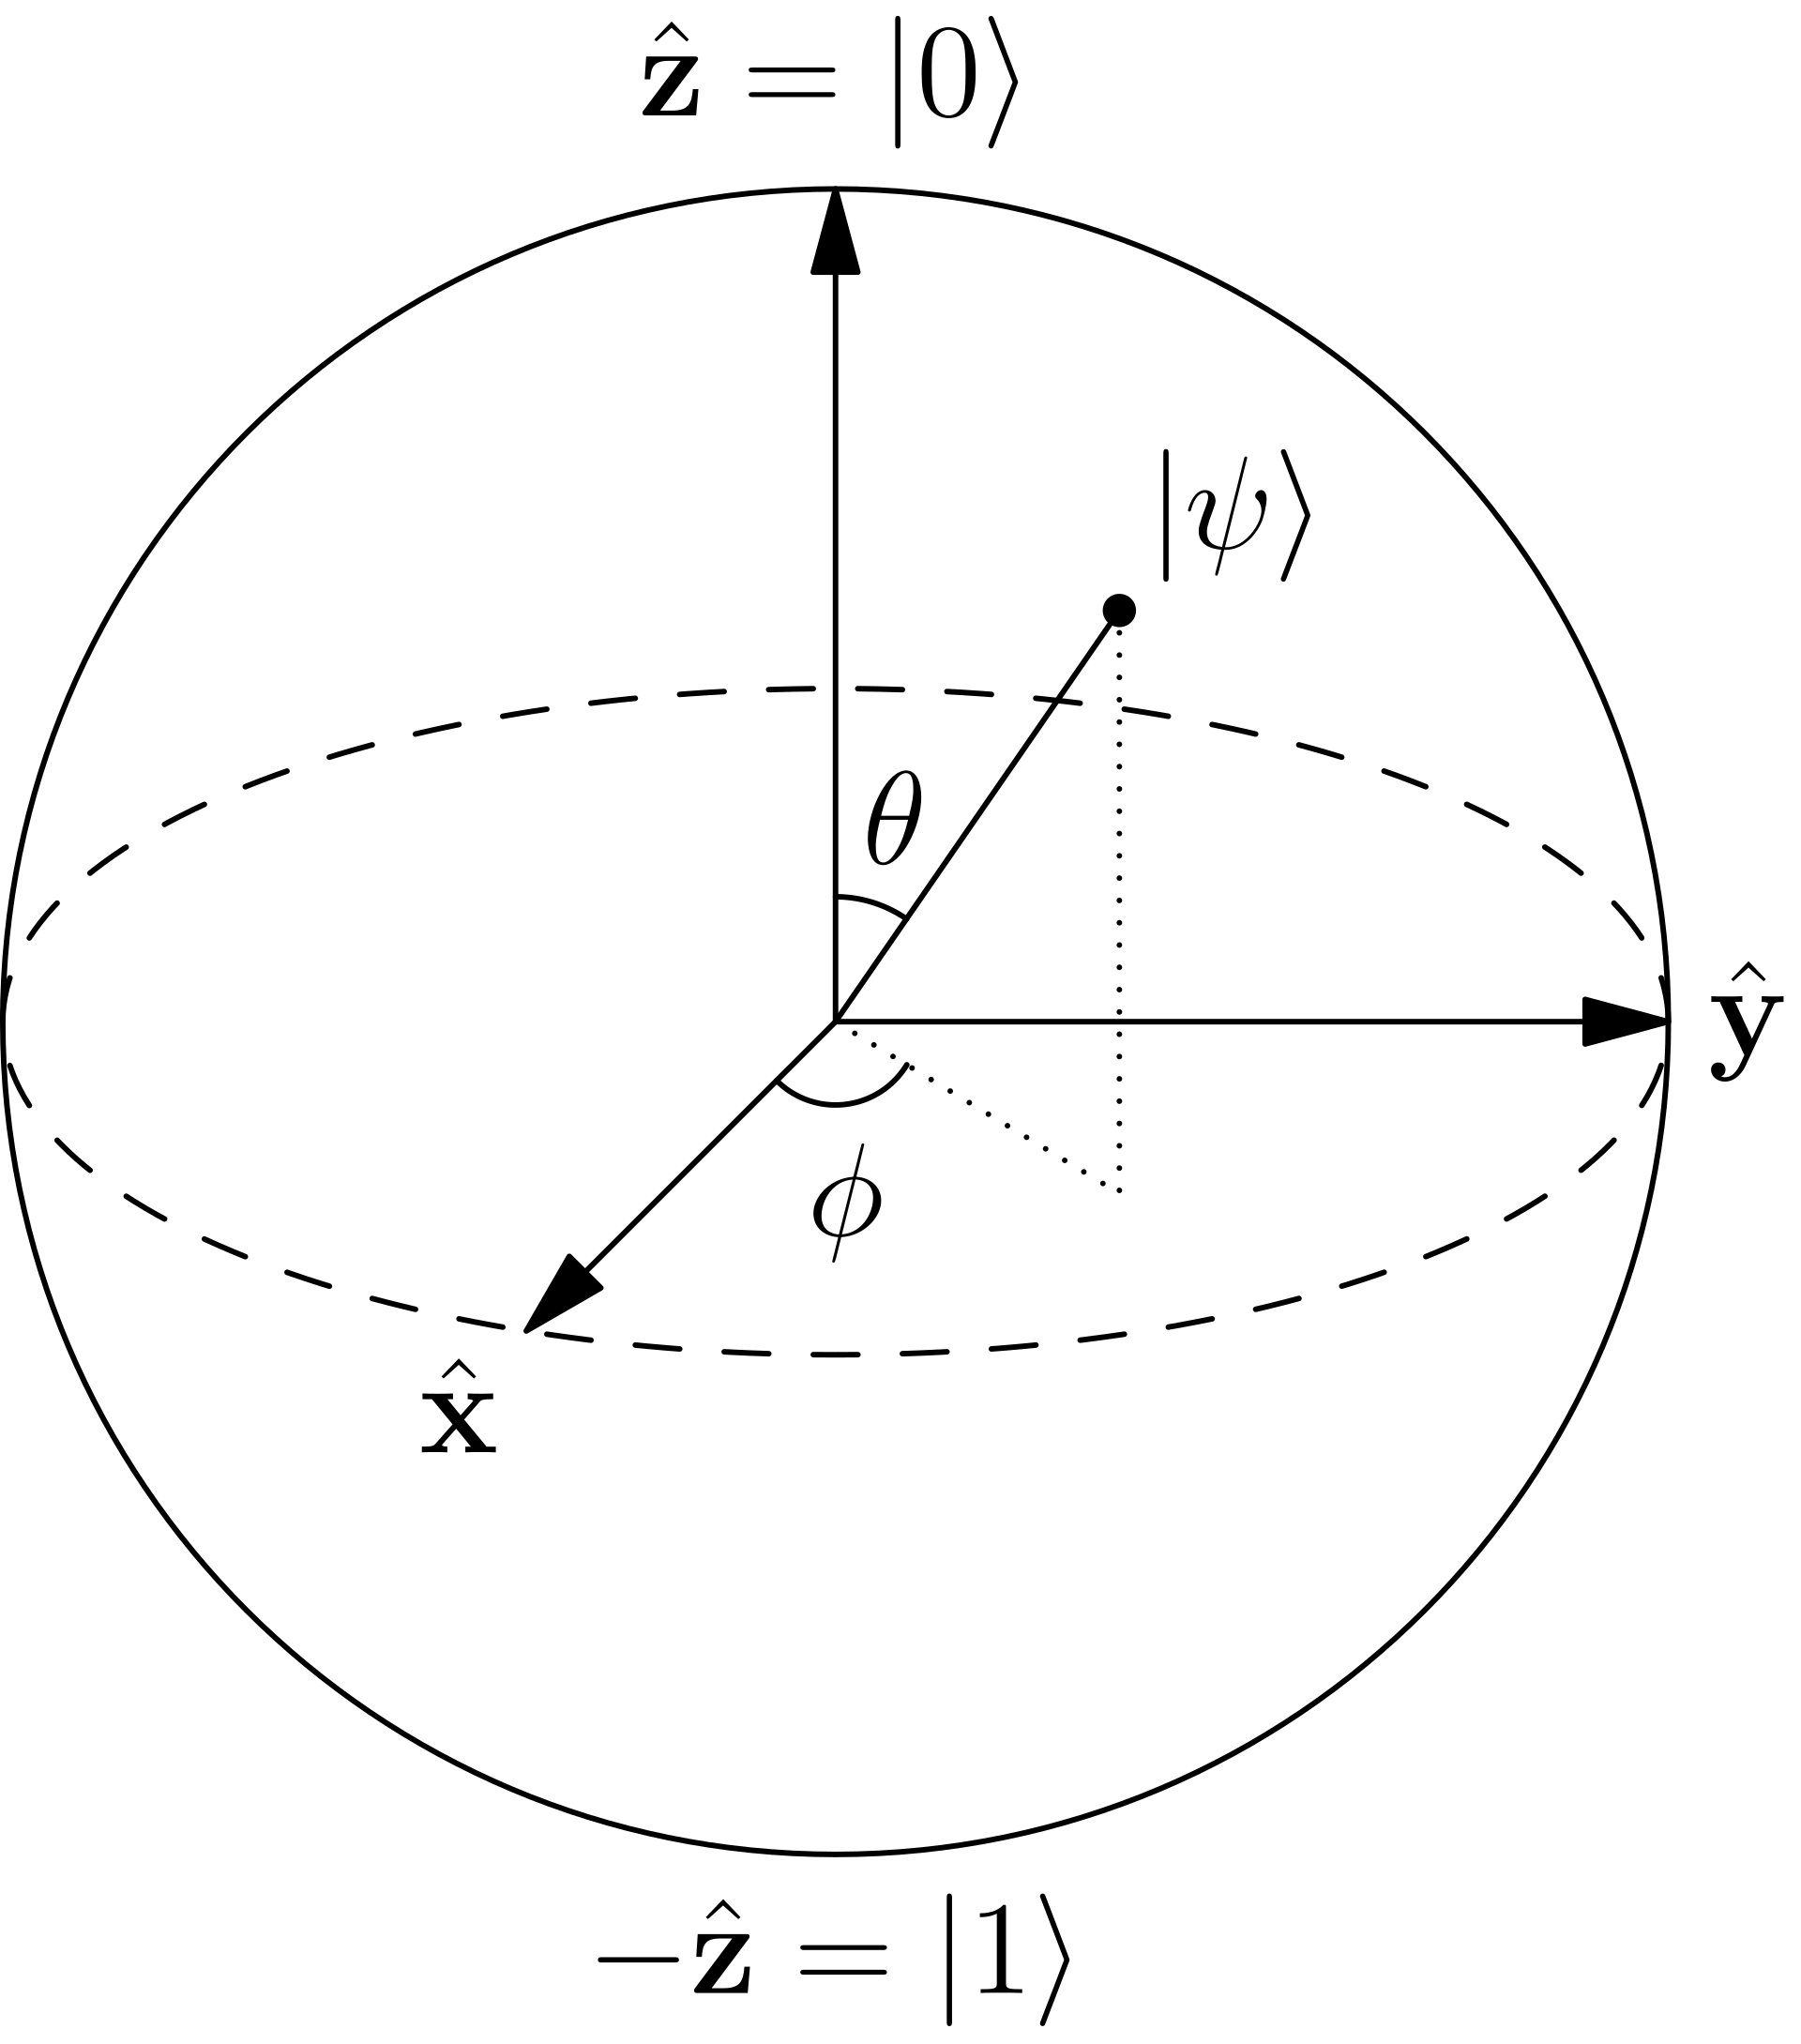
\includegraphics[width = 0.3\textwidth]{Abbildungen/Bloch_sphere_wikimedia.png}
    \caption{Schematischer Aufbau einer Bloch-Sphäre. Dabei entspricht $|0\rangle$  gerade $|\uparrow\rangle$ und $|1\rangle$ gerade 
    $|\downarrow\rangle$ \cite{pict}.}
    \label{fig:qubit}
\end{wrapfigure}
Zur Vereinfachung werden alle Kernspins (wie der Elektronenspin) als 1/2-Spins angenommen. 
Wir nutzen die Geometrie des 1/2-Spins aus und verwenden zur Darstellung die bekannte \textbf{Bloch-Sphäre}. 
Ähnlich wie die komplexe e-Funktion dank trigonometrischer Eigenschaften einen Kreis auf der Zahlenebene abbilden kann, ist es auch möglich,
jeden Punkt auf einer Kugeloberfläche zu beschreiben. Die folgende Wellenfunktion 
\begin{align}\label{klassischer_Ansatz}
    \ket{\Psi(\mu_1(t),...,\mu_n(t))} &= \frac{1}{N}\prod_{i=1}^{n} e^{\mu_i\thinspace S_i^-}\ket{\uparrow,...,\uparrow}
\end{align}
mit dem Normierungsfaktor
\begin{align}
    N &= \prod_{i=1}^{n} \frac{1}{\sqrt{1+\mu_i\muk_i}}.
\end{align}
beschreibt gerade einen Produktzustand aus $n$ Bloch-Sphären und wird mit den komplexen Parametern $\mu_i(t)$ parametrisiert. Dabei beschreibt der
Betrag $|\mu|$ die Anteile von $|\uparrow\rangle$ und $|\downarrow\rangle$ in der Wellenfunktion jeweils. Der Zustand $|\uparrow\rangle$ kann durch $\mu=0$ 
und der Zustand $|\downarrow\rangle$ als Grenzwert für $|\mu|\rightarrow \infty$ erreicht werden; dadurch steht der Betrag $|\mu|$ in Beziehung mit
mit dem Winkel $\theta$ in \autoref{fig:qubit} über $\theta = 2\tan^{-1}(|\mu|)$. Das komplexe Argument von $\mu$ beschreibt dabei die Phase der 
Zustände und steht deshalb ebenfalls in Beziehung mit dem Winkel $\phi$ in \autoref{fig:qubit}.\\
Dieser Ansatz ist die Basis für weitere Korrekturen, die im späteren Verlauf verwendet werden können, um quantenmechanische Effekte berücksichtigen zu 
können.\\
Es wird der Ansatz aus Gl. (\ref{klassischer_Ansatz}) ohne den Normierungsfaktor verwendet, da das TDVP nur eine analytische Wellenfunktion variieren kann,
der Normierungsfaktor ist aber durch das Auftauchen von $\mu_i$ und dem konjugierten $\muk_i$ nicht analytisch. Es kann aber immer noch auf die 
verallgemeinerte Euler-Lagrange-Gleichungen Gl. (\ref{verallgemeinerter_Euler_Lagrange}) zurückgegriffen werden.\\
%%%%%%%%%
%%%%%%%%%
\section{Spin-1/2 im konstanten Magnetfeld}
Zum besseren Verständnis des TDVPs ist die beispielhafte Betrachtung des vereinfachten Falles sehr aufschlussreich. 
Zudem lassen sich Identitäten herleiten, die in die Erweiterung zum \textbf{Zentralspinmodell} Wiederverwendung finden werden. Hierfür wird nur der erste 
Summand des Zentralspinmodells betrachtet bzw. der Hamilton-Operator für einen Spin in einem Magnetfeld:
\begin{align}
    \hat{H}_1 &= \vec{b}\hat{\vec{S}} = \left(b_x\hat{S}_x+b_y\hat{S}_y+b_z\hat{S}_z \right) \\
    &= \frac{b_x}{2}\Bigl(\ket{\downarrow}\!\bra{\uparrow}+\ket{\uparrow}\!\bra{\downarrow}\Bigr) \\
    & + \frac{ib_y}{2}\Bigl(\ket{\downarrow}\!\bra{\uparrow}-\ket{\uparrow}\!\bra{\downarrow}\Bigr) \\
    & + \frac{b_z}{2}\Bigl(\ket{\uparrow}\!\bra{\uparrow}-\ket{\downarrow}\!\bra{\downarrow}\Bigr), 
\end{align}
\noindent wobei der Lande-Faktor des freien Elektrones $g_e\approx 2$ ist. 
Der Spin-Vektororperator hat die Form $\hat{\vec{S}}= \frac{1}{2}\left(\hat{\sigma}_x,\hat{\sigma}_y,\hat{\sigma}_z\right)^T$ mit den Pauli-Matrizen 
$\hat{\sigma}_i$. Aus dem klassichen Ansatz Gl. (\ref{klassischer_Ansatz}) ergibt sich
\begin{align*}
    \ket{\Psi} &= e^{\mu\thinspace S^-}\ket{\uparrow} \\
            &= (1 + \frac{\mu\thinspace S^{-}}{1!} + \frac{\left(\mu\thinspace S^{-}\right)^2}{2!} + ...)\ket{\uparrow}    \\
            &= \ket{\uparrow} + \mu\ket{\downarrow}.
\end{align*}
\noindent Dabei haben wurde die Eigenschaft des 1/2-Spins $\left(S^{-}\right)^{n}\ket{\uparrow}=0$  (n = 2,3,...) verwendet.
Dieser Ansatz deckt unter Berücksichtigung der Normierung und der Phasenfreiheit den gesamten Hilbertraum des 1/2-Spins ab
\begin{align}
    \ket{\mu} &= e^{i\phi}\frac{1}{\sqrt{1 + \mu\muk}}\ket{\uparrow} + e^{i\phi}\frac{\mu}{\sqrt{1 + \mu\muk}}\ket{\downarrow}.
\end{align} 
Somit ergibt sich der effektive Hamilton-Funktion und seine partielle Ableitung nach $\muk$:
\begin{align}
    \mathcal{H} &= \frac{1}{2}\frac{b_x(\mu +\muk) + ib_y(\muk - \mu) + b_z(1-\mu\muk) }{1+\mu\muk}    \\
    \partial_{\muk} \mathcal{H} &= \frac{1}{2} \frac{b_x(1-\mu^2) + ib_y(1+\mu^2) - 2\mu b_z}{(1+\mu\muk)^2} .
\end{align}
\noindent Im nächsten Schritt wird die von dem Hamiltionian unabhängige modifizierte Gram-Matrix $G_{ij}$ bestimmt, 
welche in diesem Fall eindimesnional ist.
Damit erhalten wir
\begin{align}
    G_{11} = \frac{1}{\left(1 + \mu\overline{\mu}\right)^2} \text{\space\space bzw.\space\space } G_{11}^{-1} = \left(1 + \mu\overline{\mu}\right)^2 .
\end{align}
\noindent Einsetzen in die verallgemeinerte Euler-Lagrange-Gleichung Gl. (\ref{verallgemeinerter_Euler_Lagrange}) liefert:
\begin{align}
    i\dot{\mu} &=  \left(G_{11}\right)^{-1}\partial_{\muk} \mathcal{H} = \frac{b_x}{2}(1-\mu^2) + \frac{i b_y }{2}(1+\mu^2) -\mu b_z\label{Larmor}\\
    \leftrightarrow \dot{\mu} &= \frac{ b_y }{2}(1+\mu^2) - \frac{ib_x}{2}(1-\mu^2)   + i\mu b_z .
\end{align}
Die normierten \textbf{Spin-Erwartungswerte} $\frac{\bra{\Psi}\hat{\vec{S}}\ket{\Psi}}{\N}$ lauten:
\begin{align}
    \frac{\bra{\Psi}\hat{S_x}\ket{\Psi}}{\N} &= \frac{1}{2}\frac{\muk + \mu}{1+\mu\muk} = \frac{Re[\mu]}{1 + \mu\muk} \\
    \frac{\bra{\Psi}\hat{S_y}\ket{\Psi}}{\N} &= \frac{i}{2}\frac{\muk - \mu}{1+\mu\muk} = \frac{Im[\mu]}{1 + \mu\muk} \\
    \frac{\bra{\Psi}\hat{S_z}\ket{\Psi}}{\N} &= \frac{1}{2}\frac{1 - \mu\muk}{1 + \mu\muk}  .
\end{align}
Unter Verwendung der Identität 
\begin{align}
    \frac{d}{dt}\left(\frac{\bra{\Psi}\hat{S_\alpha}\ket{\Psi}}{\N}\right) &= \partial_{\mu}\left[\frac{\bra{\Psi}\hat{S_\alpha}\ket{\Psi}}{\N}\right]\dot{\mu} 
    + \partial_{\muk}\left[\frac{\bra{\Psi}\hat{S_\alpha}\ket{\Psi}}{\N}\right]\dot{\muk}\label{dS_dt}
\end{align}
lassen sich die Bewegungsgleichungen der Spinerwartungswerte berechnen. Für $S_x$ ergibt sich:
\begin{flalign}
    \frac{d}{dt}\left(\frac{\bra{\Psi}\hat{S_x}\ket{\Psi}}{\N}\right) =& \frac{1}{2}\frac{1-\muk^2}{(1+\mu\muk)^2}\cdot\left[\frac{ b_y }{2}(1+\mu^2) - \frac{ib_x}{2}(1-\mu^2)   + i\mu b_z\right] \nonumber \\
    &+ \frac{1}{2}\frac{1-\mu^2}{(1+\mu\muk)^2}\cdot\left[\frac{ b_y }{2}(1+\muk^2) + \frac{ib_x}{2}(1-\muk^2)   - i\muk b_z\right]  \nonumber \\
    =& \frac{1}{2(1+\mu\muk)^2}\bigg(\frac{b_y}{2}\underbrace{[(1-\muk^2)(1+\mu^2) + (1-\mu^2)(1+\muk^2)]}_{=2(1-\mu\muk)(1+\mu\muk)} \nonumber \\
    &- \frac{ib_x}{2}\underbrace{\left[(1-\muk^2)(1-\mu^2) - (1-\mu^2)(1-\muk^2)\right]}_{=0}     \nonumber \\
    &+ ib_z\underbrace{\left[\mu(1-\muk^2) -\muk(1-\mu^2) \right]}_{=-(\muk - \mu)(1+\mu\muk)}      \bigg)                         \nonumber \\    
    =& b_y \frac{1}{2}\frac{1-\mu\muk}{(1+\mu\muk)} - b_z \frac{i}{2}\frac{\muk -\mu}{(1+\mu\muk)}  \nonumber  \\
    =& b_y\left(\frac{\bra{\Psi}\hat{S_z}\ket{\Psi}}{\N}\right) - b_z\left(\frac{\bra{\Psi}\hat{S_x}\ket{\Psi}}{\N}\right).
\end{flalign}
Für $S_y$:
\begin{flalign}
    \frac{d}{dt}\left(\frac{\bra{\Psi}\hat{S_y}\ket{\Psi}}{\N}\right) =& -\frac{i}{2}\frac{1+\muk^2}{(1+\mu\muk)^2}\cdot\left[\frac{ b_y }{2}(1+\mu^2) - \frac{ib_x}{2}(1-\mu^2)   + i\mu b_z\right] \nonumber \\
    &+ \frac{i}{2}\frac{1+\mu^2}{(1+\mu\muk)^2}\cdot\left[\frac{ b_y }{2}(1+\muk^2) + \frac{ib_x}{2}(1-\muk^2)   - i\muk b_z\right]  \nonumber \\
    =& \frac{i}{2(1+\mu\muk)^2}\bigg(\frac{b_y}{2}\underbrace{[(1+\muk^2)(1+\mu^2) - (1+-\mu^2)(1+\muk^2)]}_{=0} \nonumber \\
    &+ \frac{ib_x}{2}\underbrace{\left[(1+\muk^2)(1-\mu^2) + (1-\mu^2)(1+\muk^2)\right]}_{=2(1-\mu\muk)(1+\mu\muk)}     \nonumber \\
    &+ ib_z\underbrace{\left[\mu(1-\muk^2) -\muk(1-\mu^2) \right]}_{=-(\muk + \mu)(1+\mu\muk)}      \bigg)                         \nonumber \\    
    =& -b_x \frac{1}{2}\frac{1-\mu\muk}{(1+\mu\muk)} + b_z \frac{1}{2}\frac{\muk +\mu}{(1+\mu\muk)}  \nonumber  \\
    =& b_z\left(\frac{\bra{\Psi}\hat{S_x}\ket{\Psi}}{\N}\right) - b_x\left(\frac{\bra{\Psi}\hat{S_z}\ket{\Psi}}{\N}\right).
\end{flalign}
Für $S_z$:
\begin{flalign}
    \frac{d}{dt}\left(\frac{\bra{\Psi}\hat{S_z}\ket{\Psi}}{\N}\right) =& -\frac{\muk}{(1+\mu\muk)^2}\cdot\left[\frac{ b_y }{2}(1+\mu^2) - \frac{ib_x}{2}(1-\mu^2)   + i\mu b_z\right] \nonumber \\
    &- \frac{\mu}{(1+\mu\muk)^2}\cdot\left[\frac{ b_y }{2}(1+\muk^2) + \frac{ib_x}{2}(1-\muk^2)   - i\muk b_z\right]  \nonumber \\
    =& \frac{1}{(1+\mu\muk)^2}\bigg(\frac{b_y}{2}\underbrace{[\muk(1+\mu^2) + \mu(1+\muk^2)]}_{=(\mu + \muk)(1 + \mu\muk)} \nonumber \\
    &+ \frac{ib_x}{2}\underbrace{\left[\mu(1-\muk^2) - \muk(1-\mu^2)\right]}_{=-(\muk-\mu)(1+\mu\muk)}     \nonumber \\
    &+ ib_z\underbrace{\left[\muk\mu - \mu\muk \right]}_{=0}      \bigg)                         \nonumber \\    
    =& b_x \frac{i}{2}\frac{\muk-\mu}{(1+\mu\muk)} - b_y \frac{1}{2}\frac{\muk +\mu}{(1+\mu\muk)}  \nonumber  \\
    =& b_x\left(\frac{\bra{\Psi}\hat{S_y}\ket{\Psi}}{\N}\right) - b_y\left(\frac{\bra{\Psi}\hat{S_x}\ket{\Psi}}{\N}\right).
\end{flalign}
Zusammenfassend ergibt sich:
\begin{align}
    \frac{d}{dt}\left(\frac{\bra{\Psi}\hat{\vec{S}}\ket{\Psi}}{\N}\right) &= \vec{b} \cross \left(\frac{\bra{\Psi}\hat{\vec{S}}\ket{\Psi}}{\N}\right).
\end{align}
Dies entspricht wie zu erwarten der \textit{Larmor-Präzession}.
%%%%%%%%%%%%%%%%%%%%%%%%%%%%%%%%%%%%
\section{Zwei Spins: Klassischer Ansatz}
Der vollständige zwei 1/2-Spin-Hilbertraum wird aufgespannt durch
\begin{align}
    \ket{\Psi} &= \alpha_1\ket{\uparrow\uparrow} + \alpha_2 \ket{\downarrow\uparrow} + \alpha_3\ket{\downarrow\uparrow} + \alpha_4\ket{\downarrow\downarrow}
\end{align}
mit den unabhängigen, komplexen Parametern $\alpha_i$.
\noindent Mit dem klassischen Ansatz $\ket{\Psi} = \ket{\Psi(\mu_1, \mu_2)}$ aus Gl. (\ref{klassischer_Ansatz}) ergibt sich: 
\begin{align}
    \ket{\Psi} &= e^{\mu_1 \hat{S}^{-}}e^{\mu_2 \hat{I}^{-}}\ket{\uparrow,\uparrow} \nonumber\\
                &= \ket{\uparrow \uparrow} +\mu_1\ket{\downarrow \uparrow} + \mu_2\ket{\uparrow \downarrow} + \mu_1\mu_2\ket{\downarrow\downarrow}\nonumber\\
                &= \underbrace{\left(\ket{\uparrow}_1 + \mu_1\ket{\downarrow}_1\right)}_{\ket{\Psi_1}}\underbrace{\left(\ket{\uparrow}_2 + \mu_2\ket{\downarrow}_2\right)}_{\ket{\Psi_2}}  .
\end{align}
Dabei wurde $\hat{S}_1^{-} = \hat{S}^{-}$ und $\hat{S}_2^{-} = \hat{I}^{-}$ gesetzt, um die Unterscheidung zwischen Elektronen- und Kernspin hervorzuheben.
Wird die Phasenfreiheit und die Normierung berücksichtigt und unter einem komplexen Parameter $\mu_0$ zusammengefasst
\begin{align}\label{ueberlapp_klassisch}
    \underbrace{Ne^{i\phi}}_{=\mu_0}\ket{\Psi} &= \underbrace{\mu_0}_{\alpha_1}\ket{\uparrow \uparrow} 
    + \underbrace{\mu_0\mu_1}_{\alpha_2}\ket{\downarrow \uparrow} + \underbrace{\mu_0\mu_2}_{\alpha_3}\ket{\uparrow \downarrow} 
    + \underbrace{\mu_0\mu_1\mu_2}_{\alpha_4}\ket{\downarrow\downarrow},
\end{align}
lässt sich erkennen, dass $\alpha_1$,$\alpha_2$ und $\alpha_3$ unabhängig sind, aber $\alpha_4$ gerade 
von $\alpha_1$,$\alpha_2$ und $\alpha_3$ abhängig ist. Dadurch wird der Hilbertraum auf einen Unterraum beschränkt. Der Hamiltonoperator 
des Zentralspinmodells für den zwei 1/2-Spin Fall lautet
\begin{align}\label{zweiSpinHamilton}
    \hat{H}_{CSM} &= \vec{b}\hat{\vec{S}} +  z\vec{b}\hat{\vec{I}} + \alpha \hat{\vec{S}}\hat{\vec{I}}\space.
\end{align}
Damit ergibt sich für die effektive Hamilton-Funktion: 
\begin{align}
    \mathcal{H} &= \frac{\bra{\Psi}\hat{H}_1\ket{\Psi}+ \bra{\Psi}\hat{H}_2\ket{\Psi} +\bra{\Psi}\hat{H}_3\ket{\Psi}}{\N}
\end{align}
mit
\begin{align}
   \bra{\Psi}\hat{H_1}\ket{\Psi} &= \frac{1}{2}(1+\mu_2\muk_2)\left(b_x(1-\mu_1^2) + ib_y(1+\mu_1^2) - 2\mu_1 b_z\right)\\
   \bra{\Psi}\hat{H_2}\ket{\Psi} &= \frac{z}{2}(1+\mu_1\muk_1)\left(b_x(1-\mu_2^2) + ib_y(1+\mu_2^2) - 2\mu_2 b_z\right)\\
   \bra{\Psi}\hat{H}_3\ket{\Psi} &= \frac{\alpha}{4}\left[( \mu_1 + \muk_1)( \mu_2 + \muk_2) - (\mu_1-\muk_1)(\mu_2 - \muk_2) + (1-\mu_1\muk_1)(1-\mu_2\muk_2)\right]
\end{align}  
Und wir erhalten die partiellen Ableitungen:
\begin{align}
    \partial_{\muk_1}\mathcal{H} =& \underbrace{\frac{1}{2(1+\mu_1\muk_1)^2}[b_x(1-\mu_1^2) + ib_y(1+\mu_1^2) - b_z\mu_1]}_{= \partial_{\muk_1} \frac{\bra{\Psi}\hat{H}_1 + \hat{H}_2\ket{\Psi}}{\N}} \nonumber\\
    &+ \underbrace{\frac{\alpha}{2}\frac{(\mu_2 -\mu_1)(1+\mu_1\muk_2)}{(1+\mu_1\muk_1)^2(1+\mu_2\muk_2)}}_{= \partial_{\muk_1} \frac{\bra{\Psi}\hat{H}_3\ket{\Psi}}{\N}}\\
    \partial_{\muk_2}\mathcal{H} =& \underbrace{\frac{z}{2(1+\mu_2\muk_2)^2}[b_x(1-\mu_2^2) + iB_y(1+\mu_2^2) - B_z\mu_2]}_{= \partial_{\muk_2} \frac{\bra{\Psi}\hat{H}_1 + \hat{H}_2\ket{\Psi}}{\N}} \nonumber \\
    &+ \underbrace{\frac{\alpha}{2}\frac{(\mu_1 -\mu_2)(1+\mu_2\muk_1)}{(1+\mu_1\muk_1)(1+\mu_2\muk_2)^2}}_{= \partial_{\muk_2} \frac{\bra{\Psi}\hat{H}_3\ket{\Psi}}{\N}}\space .
\end{align}
Zudem ergibt sich die modifizierte Gram-Matrix
\begin{align}
    G &=
    \begin{pmatrix}
        (1+\mu_1\muk_1)^2 & 0 \\
        0 &(1+\mu_2\muk_2)^2
    \end{pmatrix} \\
    G^{-1} &=
    \begin{pmatrix}
        \frac{1}{(1+\mu_1\muk_1)^2} & 0 \\
        0 &\frac{1}{(1+\mu_2\muk_2)^2}
    \end{pmatrix}\space ,
\end{align}
die diesmal zweidimensional ist.
\noindent Nun können die Euler-Lagrange-Gleichungen aufgestellt werden:
\begin{align}
    i\dot{\mu}_1 &= \sum_{j}\left(G_{1j}\right)^{-1}\thinspace \partial_{\overline{\mu_j}}\mathcal{H}  \\
    &=\underbrace{\frac{1}{2}b_x(1-\mu_1^2) + \frac{i}{2}b_y(1+\mu_1^2) -\mu_1 b_z}_{\text{Ein-Spin-Präzession um } \vec{b}} +\underbrace{\frac{\alpha}{2} \frac{(\mu_2-\mu_1)(1+\mu_1\muk_2)}{1+\mu_2\muk_2}}_{\text{Ein-Spin-Präzession um } \frac{\bra{\Psi}\hat{\vec{I}}\ket{\Psi}}{\N}  } \label{DGL_klassisch_S}   
\end{align}
und in analoger Weise 
\begin{align}
    i\dot{\mu}_2 &= \underbrace{\frac{z}{2}b_x(1-\mu_2^2) + \frac{iz}{2}b_y(1+\mu_2^2) -\mu_2 z b_z}_{\text{Ein-Spin-Präzession um } \vec{b}} +\underbrace{\frac{\alpha}{2} \frac{(\mu_1-\mu_2)(1+\mu_2\muk_1)}{1+\mu_1\muk_1}}_{\text{Ein-Spin-Präzession um } \frac{\bra{\Psi}\hat{\vec{S}}\ket{\Psi}}{\N}  }.\label{DGL_klassisch_I}
\end{align}
\noindent Aufgrund der Linearität der Differentialgleichungen ist beim Vergleich mit Gl. (\ref{Larmor}) zu erkennen, dass es sich bei den ersten
beiden Summanden um die Lösung aus dem Ein-Spin-Fall im Magnetfeld handelt. Nun fehlt es noch zu beweisen, dass der letztere Summand tatsächlich die 
Präzession um den Spin-Erwartungswert des jeweilig anderen Spins beschreibt bzw. das Overhausener Feld. Dies kann gezeigt werden, wenn in 
der Gl. (\ref{Larmor}) die $b_{x,y,z}$ durch $\alpha\frac{\bra{\Psi}\hat{I}_{x,y,z}\ket{\Psi}}{\N}$ ausgetauscht
werden
\begin{align}
     \frac{\alpha}{2}\left[\underbrace{\frac{1}{2}\frac{\mu_2 + \muk_2}{1+\mu_2\muk_2}}_{\frac{\bra{\Psi}\hat{I}_x\ket{\Psi}}{\N}}(1-\mu_1^2) 
     + i \underbrace{\frac{i}{2}\frac{\muk_2 -\mu_2}{1+\mu_2\muk_2}}_{\frac{\bra{\Psi}\hat{I}_y\ket{\Psi}}{\N}}(1+\mu_1^2) 
     - 2\mu_1\underbrace{\frac{1}{2}\frac{1-\mu_2\muk_2}{1+\mu_2\muk_2}}_{\frac{\bra{\Psi}\hat{I}_z\ket{\Psi}}{\N}} \right],
\end{align}
denn einfaches Auflösen führt ebenfalls zu
\begin{align}
    \frac{\alpha}{2} \frac{(\mu_2-\mu_1)(1+\mu_1\muk_2)}{1+\mu_2\muk_2}.
\end{align}
Hier lässt sich erkennen, dass die $\alpha\frac{\bra{\Psi}\hat{I_i}\ket{\Psi}}{\N}$ die Rolle des Magnetfeldes $\vec{b}$ in der Ein-Spin-Lösung 
übernehmen. Wir erhalten dann aus Symmetriegründen:
\begin{align}
    \frac{d}{dt}\left[\frac{\bra{\Psi}\hat{\vec{S}}\ket{\Psi}}{\N}\right] &= \left(\vec{b} + \alpha \frac{\bra{\Psi}\hat{\vec{I}}\ket{\Psi}}{\N}\right)\cross\frac{\bra{\Psi}\hat{\vec{S}}\ket{\Psi}}{\N} \label{DGL_1}\\
    \frac{d}{dt}\left[\frac{\bra{\Psi}\hat{\vec{I}}\ket{\Psi}}{\N}\right] &= \left(z\vec{b} + \alpha \frac{\bra{\Psi}\hat{\vec{S}}\ket{\Psi}}{\N}\right)\cross\frac{\bra{\Psi}\hat{\vec{I}}\ket{\Psi}}{\N} \label{DGL_2}.
\end{align}


%%%%%%%%%%%%% Quantenkorrektur




\section{Modifizierter Ansatz: Quantenkorrektur}
\noindent Wie im vorherigen Abschnitt zu sehen, erhalten wir eine klassiche Lösung. Um eine genauere Lösung zu erhalten, 
führen wir einen weiteren Korrekurparameter $\mu_{12}$ ein, wodurch ein größerer Unterraum des zwei 1/2-Spin-Hilbertraumes aufgespannt 
wird, mit der Hoffnung im Gegensatz zum klassischen Ansatz die Verschränkung zu berücksichtigen. Der modifizierte Ansatz lautet:
\begin{align}
    \ket{\Psi(\mu_1,\mu_2,\mu_{12})} &= e^{\mu_1 S_1^-}e^{\mu_2 S_2^-}e^{\mu_{12} S_1^-S_2^-}\ket{\uparrow,\uparrow}\\
                                    &= \ket{\uparrow \uparrow} +\mu_1\ket{\downarrow \uparrow} + \mu_2\ket{\uparrow \downarrow} + (\mu_1\mu_2 + \mu_{12})\ket{\downarrow \downarrow}.
\end{align}
Wird  die Phasenfreiheit und die Normierung berücksichtigt und unter einem komplexen Parameter $\mu_0$ zusammengefasst, ergibt sich
\begin{align}
    \underbrace{Ne^{i\phi}}_{=\mu_0}\ket{\Psi} &= \underbrace{\mu_0}_{\alpha_1}\ket{\uparrow \uparrow} 
    + \underbrace{\mu_0\mu_1}_{\alpha_2}\ket{\downarrow \uparrow} + \underbrace{\mu_0\mu_2}_{\alpha_3}\ket{\uparrow \downarrow} 
    + \underbrace{\mu_0(\mu_1\mu_2 + \mu_{12})}_{\alpha_4}\ket{\downarrow\downarrow}.
\end{align}
Im Gegensatz zum klassischen Ansatz lässt sich erkennen, dass alle Parameter $\alpha_i$, einschließlich $\alpha_4$, unabhängig sind. Somit ist der gesamte
Hilbertraumabgedeckt und die exakte Lösung zu erwarten.\\
Aufgrund der Tatsache, dass bei einem $\vec{b}$-Feld in beliebiger Richtung, sich die Rechnung und Ergebnisse außerordentlich verkomplizieren, ohne 
wirklich neue Erkenntnis zu bringen, wird das Magnetfeld in z-Richtung ausgerichtet. Somit vereinfacht sich der 
Hamiltonian (\ref{zweiSpinHamilton}) zu:
\begin{align}\label{Hamiltonian_Bz}
    \hat{H} &= \vec{b}\hat{\vec{S}}_z +  z\vec{b}\hat{\vec{I}}_z + \alpha \hat{\vec{S}}\hat{\vec{I}}
\end{align}
Mit diesem Ansatz erhalten wir nach längerer Rechnung den modifizierten Hamiltonian:
\begin{align}
    \mathcal{H} &= \frac{\bra{\Psi}\hat{H}_1\ket{\Psi} +\bra{\Psi}\hat{H}_2\ket{\Psi} + \bra{\Psi}\hat{H}_3\ket{\Psi}}{\N}
\end{align}
mit 
\begin{align}
    \bra{\Psi}\hat{H}_1\ket{\Psi} &=  \frac{b}{2}\left[ 1- \mu_1\muk_1 + \mu_2\muk_2 - (\mu_1 \mu_2 + \mu_{12})(\overline{\mu_1\mu_2} + \muk_{12})\right]\\
    %
    \bra{\Psi}\hat{H}_2\ket{\Psi} &=  \frac{z b}{2}\left[ 1- \mu_2\muk_2 + \mu_1\muk_1 - (\mu_1 \mu_2 + \mu_{12})(\overline{\mu_1\mu_2} + \muk_{12})\right] \\
    %
    \bra{\Psi}\hat{H}_3\ket{\Psi} &= \frac{\alpha}{4}[2(\muk_1\mu_2 + \mu_1\muk_2) + 1 - \mu_1\muk_1 - \mu_2\muk_2 + (\mu_1 \mu_2 + \mu_{12})(\overline{\mu_1\mu_2} + \muk_{12})].
\end{align}
\noindent Damit folgen für die partiellen Ableitungen nach den konjugierten Parameter
\begin{align}
    \partial_{\muk_1} \mathcal{H} =& 
    -b \frac{\mu_1(1+\mu_2\muk_2)^2 + \muk_2\mu_{12}}{\N^2}\nonumber\\
    &+z b \frac{\muk_{12}(\mu_1\mu_2 + \mu_{12})}{\N^2}\nonumber\\
    &+\frac{\alpha}{2}\frac{(\mu_2-\mu_1)(\mu_1\muk_2+1)(1+\mu_2\muk_2)+\muk_{12}(\mu_1\mu_2 + \mu_{12}) + \mu_{12}\muk_2}{\N^2}\label{dH_Q1} \\
    %
    \partial_{\muk_2} \mathcal{H} =& 
    +b \frac{\muk_{12}(\mu_1\mu_2 + \mu_{12})}{\N^2} \nonumber\\
    &-z b \frac{\mu_2(1+\mu_1\muk_1)^2 + \muk_1\mu_{12}}{\N^2} \nonumber\\
    &+\frac{\alpha}{2}\frac{(\mu_1-\mu_2)(\mu_2\muk_1+1)(1+\mu_1\muk_1)+\muk_{12}(\mu_1\mu_2 + \mu_{12}) + \mu_{12}\muk_1}{\N^2} \\
    %
    \partial_{\muk_{12}} \mathcal{H} =& 
    -b\frac{(\mu_1\mu_2+\mu_{12})(1+\mu_2\muk_2)}{\N^2} \nonumber\\
    &-zb\frac{(\mu_1\mu_2+\mu_{12})(1+\mu_1\muk_1)}{\N^2} \nonumber\\
    &+\frac{\alpha}{2}\frac{(\muk_1-\muk_2)(\mu_1-\mu_2)(\mu_1\mu_2+\mu_{12})}{\N^2}\label{dH_Q12}
\end{align}
\noindent und für die Gram-Matrix erhalten wir:
\begin{align}\label{Gram_Korrektur}
    G &=
    \begin{pmatrix}
        (1+\mu_1\muk_1)^2 + \mu_{12}\muk_{12} & -\mu_1^2\muk_{12} - \muk_2^2\mu_{12} &  \mu_2(1+\mu_2\muk_2)-\muk_1\mu_{12}\\
        -\mu_2^2\muk_{12} - \muk_1^2\mu_{12} &(1+\mu_2\muk_2)^2 + \mu_{12}\muk_{12} & \mu_1(1+\mu_1\muk_1)-\muk_2\mu_{12}\\
        \muk_2(1+\mu_2\muk_2)-\mu_1\muk_{12} & \muk_1(1+\mu_1\muk_1)-\mu_2\muk_{12} & 1 + \mu_1\muk_1 + \mu_2\muk_2
    \end{pmatrix}\frac{1}{\N^2} .
\end{align}
Somit lassen sich die Bewegungsgleichungen der Parameter explizit aufschreiben:
\begin{align}
    i\dot{\mu}_1 &= G_{1,1}^{-1}\thinspace \partial_{\muk_1}\mathcal{H} + G_{1,2}^{-1}\thinspace\partial_{\muk_2}\mathcal{H} + G_{1,3}^{-1}\thinspace\partial_{\muk_3}\mathcal{H}\label{QK_DGL1} \\
    i\dot{\mu}_2 &= G_{2,1}^{-1}\thinspace\partial_{\muk_1}\mathcal{H} + G_{3,2}^{-1\thinspace}\partial_{\muk_2}\mathcal{H} + G_{2,3}^{-1}\thinspace\partial_{\muk_3}\mathcal{H} \\
    i\dot{\mu}_{12} &= G_{3,1}^{-1}\thinspace\partial_{\muk_1}\mathcal{H} + G_{3,2}^{-1}\thinspace\partial_{\muk_2}\mathcal{H} + G_{3,3}^{-1}\thinspace\partial_{\muk_3}\mathcal{H} \label{QK_DGL3}.
\end{align}
Die Ergebnisse sind deutlich komplexer als für den klassischen Ansatz. Zur Herleitung der Spindynamik würden sich deshalb numerische Methoden zur Lösung der 
Differentialgleichung ergeben, wobei die modifizierte Gram-Matrix Gl. (\ref{Gram_Korrektur}) der Kürze halber auch numerisch invertiert werden kann, da eine 
direkte Inversion einen noch kompliziertere Matrix ergeben würde mit wenig neuer Erkenntnis.
